\documentclass{standalone}
\usepackage{pgfplots}
\pgfplotsset{compat=newest}

\begin{document}
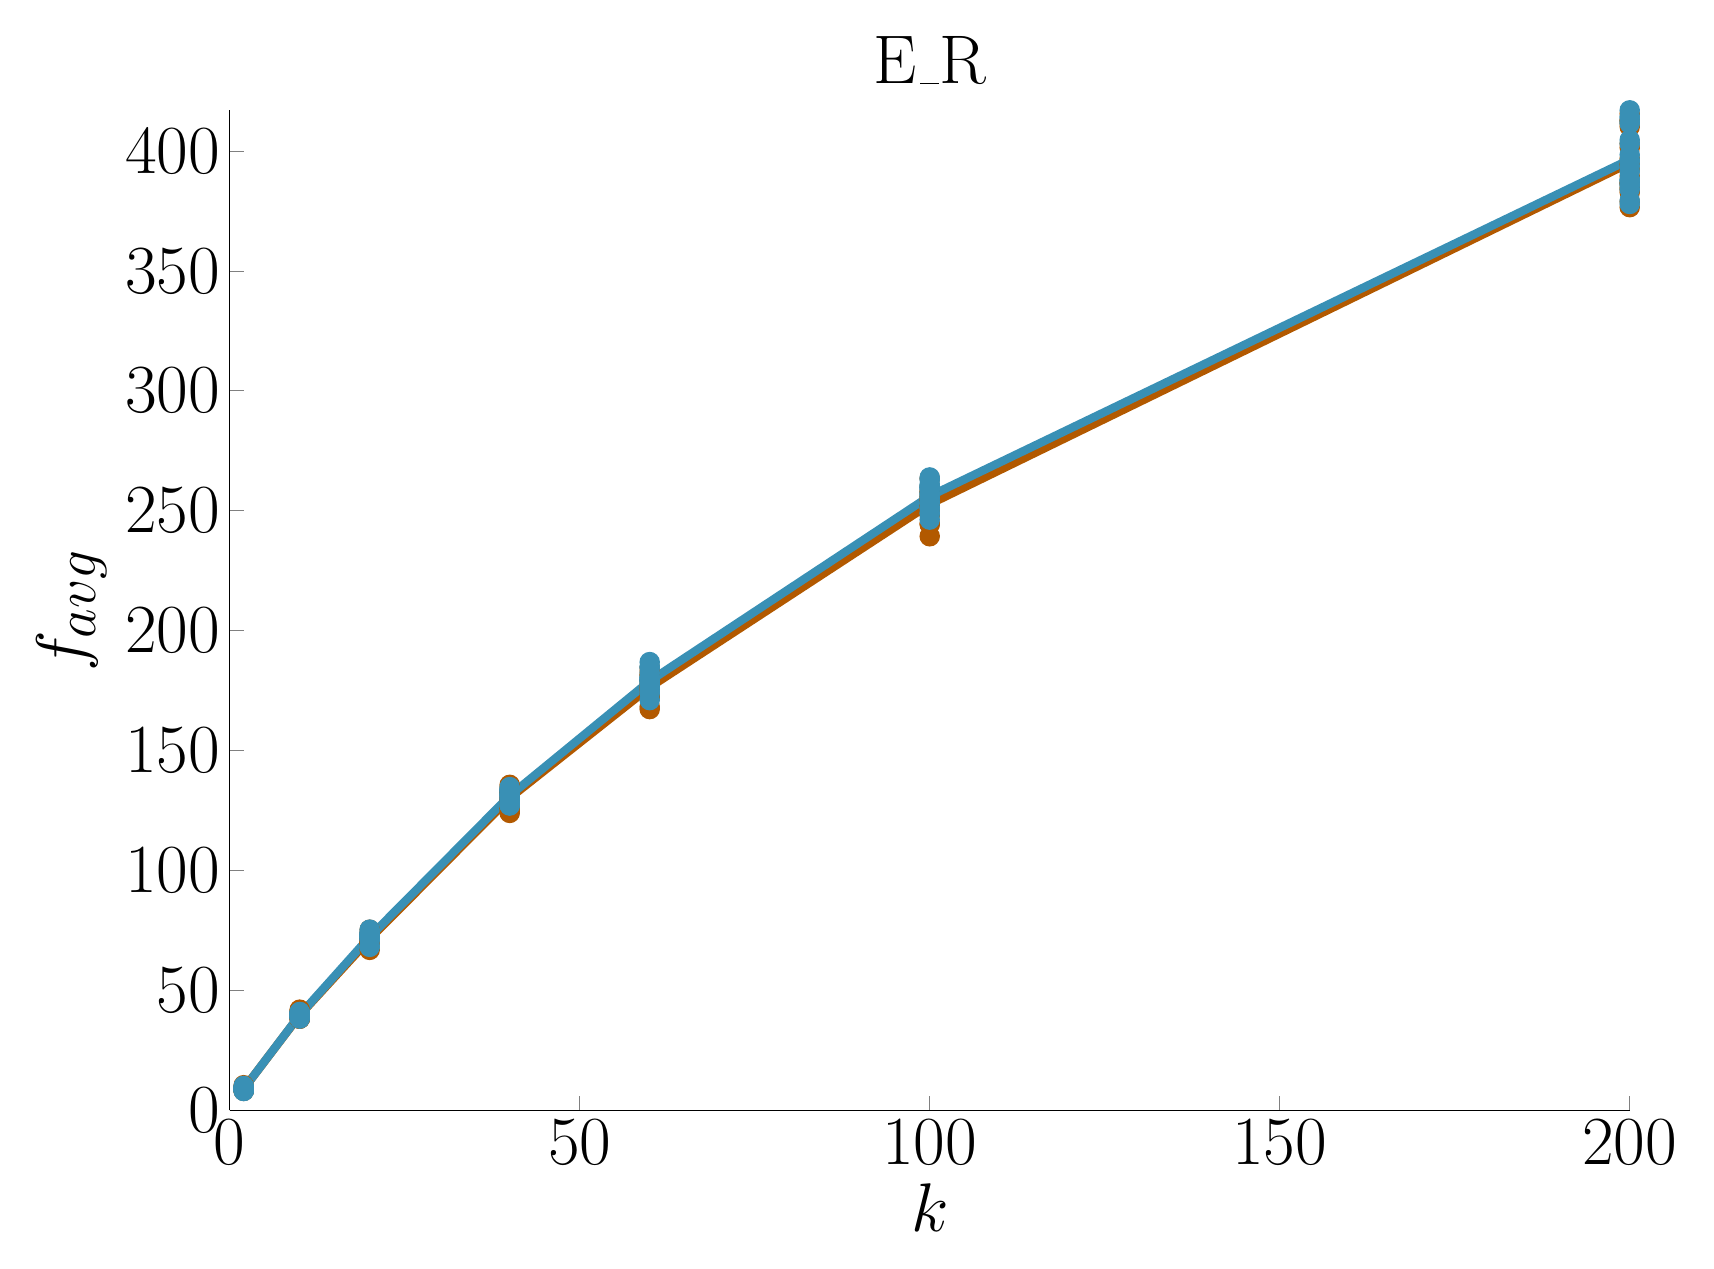
\begin{tikzpicture}

\begin{axis}[%
title style={font=\Huge},
title=E\_R,
tick label style={font=\Huge},
label style={font=\Huge},
legend style={font=\Huge},
view={0}{90},
max space between ticks=50pt,
width=7in,
height=5in,
scale only axis,
xmin=0, xmax=200,
xtick={0, 50, 100, 150, 200},
xlabel={$k$},
ymin=0, ymax=416.91,
%ytick={0, 200, 400, 600, 800, 1000},
ylabel={$f_{avg}$},
major tick length=5pt,
axis lines*=left,
legend cell align=left,
clip=false]

\addplot [
only marks,
mark=*,
mark size=3.5pt,
color=orange!70!black,
%solid,
%line width=2pt,
]
coordinates{
(2,8.11)(2,8.31)(2,8.37)(2,8.38)(2,8.42)(2,8.7)(2,8.75)(2,8.81)(2,8.9)(2,8.93)(2,8.94)(2,8.95)(2,9.04)(2,9.08)(2,9.13)(2,9.19)(2,9.29)(2,9.35)(2,9.62)(2,10.47)(10,38.2)(10,38.24)(10,38.28)(10,38.32)(10,38.33)(10,38.53)(10,38.69)(10,38.81)(10,39.22)(10,39.31)(10,39.8)(10,40.05)(10,40.09)(10,40.27)(10,40.36)(10,40.82)(10,40.93)(10,40.96)(10,41.31)(10,41.97)(20,66.88)(20,69.25)(20,69.74)(20,70.12)(20,70.37)(20,70.49)(20,70.82)(20,70.98)(20,71.09)(20,71.13)(20,71.98)(20,72.0)(20,72.01)(20,72.01)(20,72.18)(20,72.2)(20,72.78)(20,73.38)(20,74.1)(20,75.29)(40,123.98)(40,124.46)(40,125.8)(40,125.9)(40,127.6)(40,129.38)(40,129.4)(40,129.48)(40,129.72)(40,130.25)(40,130.41)(40,131.24)(40,131.92)(40,132.14)(40,132.47)(40,132.6)(40,132.79)(40,133.4)(40,134.73)(40,135.7)(60,167.27)(60,168.25)(60,172.14)(60,172.42)(60,174.01)(60,174.6)(60,174.87)(60,174.94)(60,175.0)(60,176.07)(60,176.34)(60,177.08)(60,177.3)(60,177.64)(60,179.11)(60,179.24)(60,181.32)(60,181.73)(60,183.14)(60,184.6)(100,239.32)(100,244.23)(100,244.62)(100,248.22)(100,248.28)(100,250.1)(100,251.22)(100,251.49)(100,251.58)(100,251.85)(100,254.16)(100,254.32)(100,255.21)(100,255.84)(100,256.09)(100,257.67)(100,257.8)(100,258.1)(100,260.04)(100,263.46)(200,376.52)(200,378.76)(200,382.7)(200,383.86)(200,384.66)(200,386.24)(200,386.37)(200,386.7)(200,389.54)(200,392.2)(200,394.05)(200,394.38)(200,396.82)(200,401.29)(200,402.97)(200,410.04)(200,411.54)(200,412.67)(200,412.69)(200,415.52)
};

\addplot [
only marks,
mark=*,
mark size=3.5pt,
color=cyan!70!black,
%solid,
%line width=2pt,
]
coordinates{
(2,8.04)(2,8.17)(2,8.42)(2,8.51)(2,8.55)(2,8.58)(2,8.63)(2,8.82)(2,8.88)(2,8.96)(2,8.99)(2,9.04)(2,9.06)(2,9.07)(2,9.11)(2,9.13)(2,9.29)(2,9.49)(2,9.75)(2,10.18)(10,38.22)(10,38.59)(10,38.6)(10,39.22)(10,39.34)(10,39.42)(10,39.5)(10,39.53)(10,39.54)(10,39.61)(10,39.74)(10,39.78)(10,40.01)(10,40.05)(10,40.11)(10,40.48)(10,40.56)(10,40.76)(10,40.81)(10,41.0)(20,68.13)(20,68.43)(20,71.0)(20,71.26)(20,71.75)(20,72.23)(20,72.31)(20,72.44)(20,72.46)(20,72.47)(20,72.54)(20,72.86)(20,72.88)(20,72.93)(20,73.07)(20,73.17)(20,73.4)(20,73.91)(20,74.19)(20,75.33)(40,127.06)(40,127.2)(40,127.8)(40,128.46)(40,128.59)(40,129.59)(40,129.9)(40,130.39)(40,131.32)(40,131.35)(40,131.72)(40,131.81)(40,132.0)(40,133.15)(40,133.22)(40,133.34)(40,133.82)(40,133.84)(40,133.88)(40,134.77)(60,171.0)(60,174.07)(60,174.45)(60,174.85)(60,176.05)(60,177.31)(60,177.36)(60,177.86)(60,179.02)(60,179.06)(60,179.13)(60,179.29)(60,179.81)(60,180.48)(60,180.53)(60,180.56)(60,182.44)(60,184.45)(60,184.99)(60,186.87)(100,246.25)(100,248.86)(100,249.05)(100,250.91)(100,251.48)(100,253.29)(100,253.88)(100,255.36)(100,255.4)(100,256.74)(100,256.91)(100,257.49)(100,258.89)(100,259.48)(100,259.53)(100,259.71)(100,260.58)(100,260.8)(100,262.83)(100,263.86)(200,377.86)(200,379.36)(200,383.99)(200,385.56)(200,386.3)(200,387.61)(200,387.65)(200,388.2)(200,391.43)(200,393.7)(200,395.78)(200,396.04)(200,398.36)(200,402.97)(200,404.58)(200,411.37)(200,412.36)(200,413.67)(200,414.28)(200,416.91)
};

\addplot [
color=orange!70!black,
solid,
line width=3pt
]
coordinates{
(2,8.937)(10,39.6245)(20,71.44)(40,130.1685)(60,176.3535)(100,252.68)(200,394.976)
};

\addplot [
color=cyan!70!black,
solid,
line width=3pt
]
coordinates{
(2,8.9335)(10,39.7435)(20,72.338)(40,131.1605)(60,178.979)(100,256.065)(200,396.399)
};


\end{axis}
\end{tikzpicture}
\end{document}
